\chapter{The STAR detector and RHIC collider}
\label{detector}
The relativistic heavy ion collider (RHIC) is located at Brookhaven National Laboratory (BNL) on Long Island, in the state of New York. The facilities were rebuilt after the end of World War II from a U.S. Army camp into the scientific and technological laboratory it is now. It is one of several national laboratories under the United States Department of Energy administration. 
\newline
Brookhaven National Laboratory has a long history with particle physics. The first accelerator at BNL was the Cosmotron which operated between the years of 1952 and 1966. Brookhaven was and still is home of many accelerators such as the Alternating Gradient Synchrotron, National Synchrotron Light Source I or the newest National Synchrotron Light Source II. The above mentioned RHIC began operating in 2000 and is discussed thoroughly in \autoref{RHIC}. Until the Large Hadron Collider began operation in 2010, RHIC was the highest energy collider in the world. Relativistic Heavy Ion Collider will be running until 2025, when it will be replaced by the Electron Ion Collider. The future of particle physics at BNL is discussed in \autoref{EIC}.

\section{RHIC}
\label{RHIC}
The Relativistic Heavy Ion Collider has been operating since 2000, but the work and planning has begun long before. The idea was proposed 16 years earlier~\cite{RHIChis}. RHIC is capable of accelerating protons for proton-proton collisions up to energies of 510 GeV. In nuclei nuclei collisions, the maximum energy is 200 GeV per nucleon. Generally, gold nuclei are used for collisions, but nuclei of elements such as copper, deuterium, Helium or many others have been used. The circumference of the collider is 3834 m \cite{Dehmelt}.

The largest detector at RHIC was the PHENIX detector. The name stands for Pioneering High Energy Nuclear Interaction eXperiment. The development began in 1991 and the goal of the experiment was to measure the Quark-Gluon Plasma\footnote{The Quark-Gluon Plasma is a state of matter created right after the collision of 2 nuclei, when the bonds between elementary particles quarks and gluons are overcome and for a brief moment, they are capable of moving freely. Some theories state that QGP was the only state of matter for a brief moment right after the big bang.} (QGP) and extreme states of matter. Another goal of the experiment was to measure where does the proton gets spin from \cite{PHENIX}.  PHENIX, at \autoref{df1}, is located at 8 o'clock of the RHIC circle. Data taking was done between the years of 2000 and 2016. After a couple of years of inactivity, a new project was born- sPHENIX. This updated version of PHENIX will begin operation in the year of 2023 and will continue until the end of RHIC in 2025. 

\FloatBarrier
\begin{figure}[ht]
    \centering
    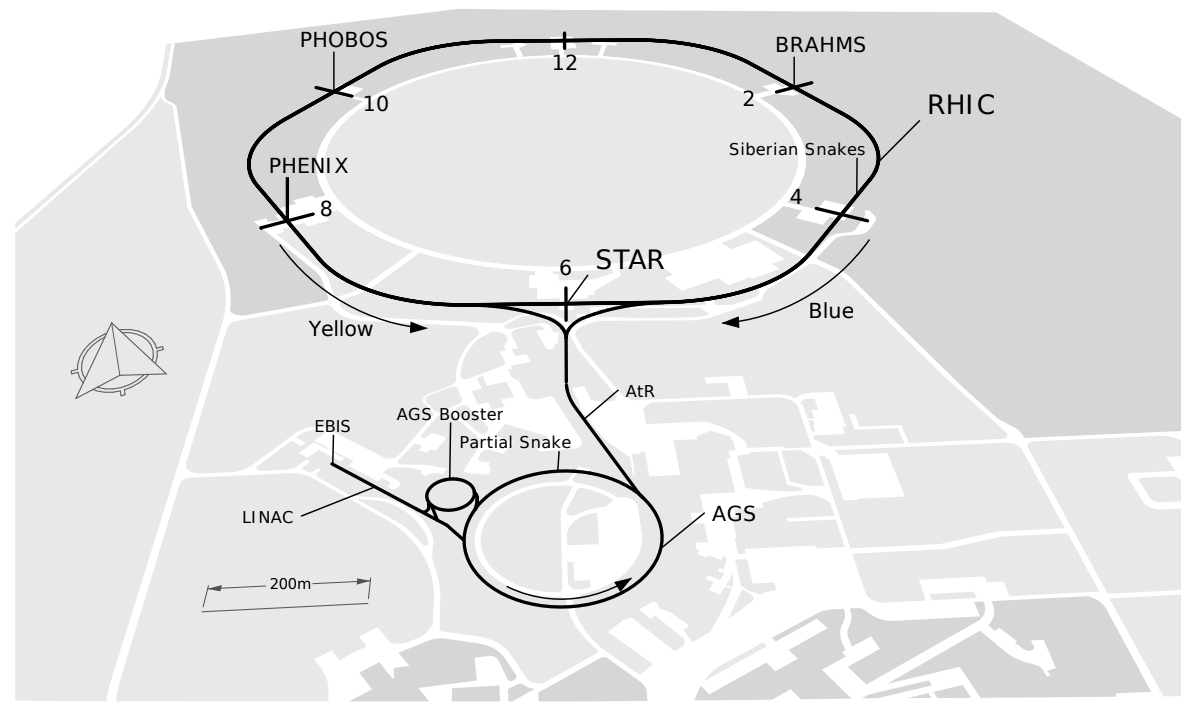
\includegraphics[width=0.9\textwidth]{figures/rhic.jpg}
    \caption[The Relativistic Heavy Ion Collider]{A sketch of the Relativistic Heavy Ion Collider with it's accelerators EBIS, Linac, AGS Booster, AGS and detectors PHENIX, PHOBOS, BRAHMS and STAR. Taken from \cite{STARgraphicsrep}. }
    \label{df1}
\end{figure}
\FloatBarrier

Next in line were PHOBOS and BRAHMS experiments. Their operating times were shorter compared to the other 2 experiments. Data taking began in 2000 and ended in 2005 at PHOBOS and 2006 at BRAHMS. PHOBOS was designed to study a large number of Au-Au collisions and create a big picture description of all sorts of events that happen during a collision. It was capable of measuring the total number of produced particles created in 1 event thanks to many silicon detectors surrounding the point of collision \cite{PHOBOS}. Even though BRAHMS was installed for the first beams in 2000, fully operational was only in 2001. The goal of the detector was to accurately identify particles with the largest possible rapidity range. The results from experiments done at BRAHMS were meant to be complimentary to measurements done at the other 3 experiments at RHIC \cite{BRAHMSadamczyk}. 
\newline
The last detector at the Relativistic Heavy Ion Collider is the STAR detector. It is located near the place at the collider, where accelerated particles enter the collider. STAR detector is the longest operating detector at RHIC. It has been operating since the beginning in 2000 and is planned to work until 2025. The entire detector consists of many subdetectors and systems, which are closely described in \autoref{STAR}. 

Particles that collide in RHIC, go through several accelerators where they gain the desired energy for collision. This is called the pre-injectory system. The source for ion beams is the Electron Beam Ion Source. It creates ion beams which are sped up by 2 small linear accelerators, that carry the beams to the Booster Synchrotron~\cite{RHIC}. For proton collisions, protons are accelerated in the Linear accelerator (Linac) which brings them to Booster. The Booster Synchrotron is able to accelerate beams of particles from 200 MeV up to around 1.2 GeV and holds the role of pre-accelerator for the Alternating Gradient Synchrotron (AGS). AGS is capable of accelerating ions from around 37 $\%$ to 99.7 $\%$ speed of light in vacuum. The synchrotron relies highly on focusing the beam of particles which increases efficiency and reduces costs of operation. The focusing is done by alternating the gradient of the magnetic field~\cite{Adams}. Accelerated ions from AGS move through AGS-to-RHIC line. At the end of the beam line is a magnet, which curves the trajectories of ions and particles either to clockwise which is the "blue" beam line, or counter clockwise direction which is the yellow beam line. Once the beams are in RHIC, they get the final acceleration kick up from radio waves, which brings the speed of ions very close to the speed of light and are ready to be collided. Particles that have been collided inside the Relativistic Heavy Ion Collider are protons, deuterons, nuclei of gold, aluminium, hydrogen, copper, zirkonium and ruthenium. 

\section{STAR detector}
\label{STAR}
The name STAR comes from the abbreviation Solenoidal Tracker At RHIC. The detector itself has gone a long way since it has been installed in 2000. Almost all parts of the detector have been upgraded or somehow improved since 2000 and several detectors have been added. This chapter discusses primarily the current STAR detector's condition, but due to lack of reliable sources, some aspects of the detector discussed in this chapter  might not be entirely up to date. 
\newline
Data for this thesis were measured in 2017, a couple years before a quite large upgrade of several detectors. The upgrade was called BES II\cite{BESII}. It focused on expanding the range of acceptance and the increasing the measuring capabilities of the forward region. Subdetectors Time Projection Chamber (TPC), Time Of Flight detector (TOF), Roman Pot system (RP), Beam Beam Counters (BBC) and Zero Degree Calorimeters (ZDC) will be discussed and some of the others will be mentioned.

\FloatBarrier
\begin{figure}[ht]
    \centering
    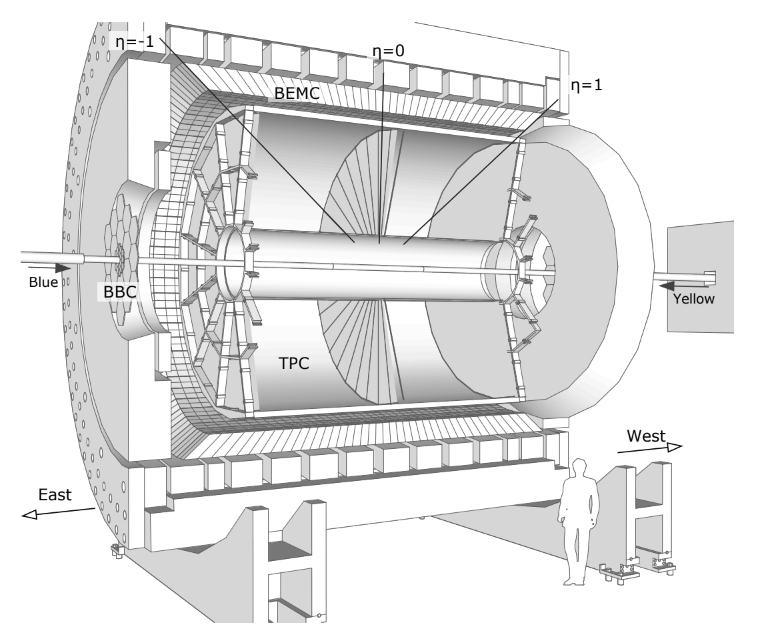
\includegraphics[width=0.65\textwidth]{figures/dete.jpg}
    \caption[Schematic view of the Solenoidal Tracker At Rhic]{A scheme of the STAR detector with names of some subdetectors. Time Projection Chamber in the middle, closest to the interaction point, around it the Barrel Electromagnetic Calorimeter. Beam Beam counters are located in the forward and backward location along the beam pipes Blue and Yellow. Taken from Ref.~\cite{dete}.}
    \label{df4}
\end{figure}
\FloatBarrier


\subsection{Time Projection Chamber}
\label{tpc}
Time Projection Chamber is located at the center of the structure. It is a cylindrical volume that surrounds the interaction point. It is 4 m wide in diameter and 4.2 m long. TPC is a ionization detector, which uses electric and magnetic field for trajectory reconstruction as well as for computing the energy loss of particles. Energy loss is extracted from the measured ionization of gas inside the chamber (90 $\%$ Argon, 10 $\%$ Methane) when electrons drift toward the anode on the sides of the cylinder. The anode is divided into several sectors. The number of sectors that detect signal from electrons then defines how well a track of a particle can be reconstructed and how precise is the energy loss computation. It is regarded in \autoref{analysis} as number of hits in TPC. The velocity of electrons defines the readout time of the detector. Ions drift toward the middle of the detector- central membrane. The drift of charged particles is caused by an electric field which is created by 3 different sources: inner field cage, outer field cage and the aforementioned central membrane\cite{STAR}. Electric field in the chamber is uniform and approximately equal to 135 V/cm \cite{TPC}. Magnetic field's operation value inside TPC is 0.5 T and is created by massive magnetic coils around the detector. The latest upgrade of TPC was BES II. The upgrade involved improving the inner TPC (iTPC) sectors for better understanding of QCD phase diagram. The improvement involved increasing the pseudorapidity by 50 $\%$ up to $|\eta|<1.5$ range, increasing the energy loss and momentum resolutions \cite{TPCupgrade}. This pseudorapidity range of detection is conditioned by a minimum value of particle's transverse momentum (150 MeV). The pad resolution was approximated between 213 and 950 $\mu$m, depending on which part of the pad the particle hits\cite{STAR} (pads are located on the cathodes and are used for reading out signal). TPC was constructed for heavy nuclei collisions which produce quite a lot of particles and fragments, therefore, it has multiplicity rate of more than 3000 tracks per event \cite{TPC}.

\FloatBarrier
\begin{figure}
    \centering
    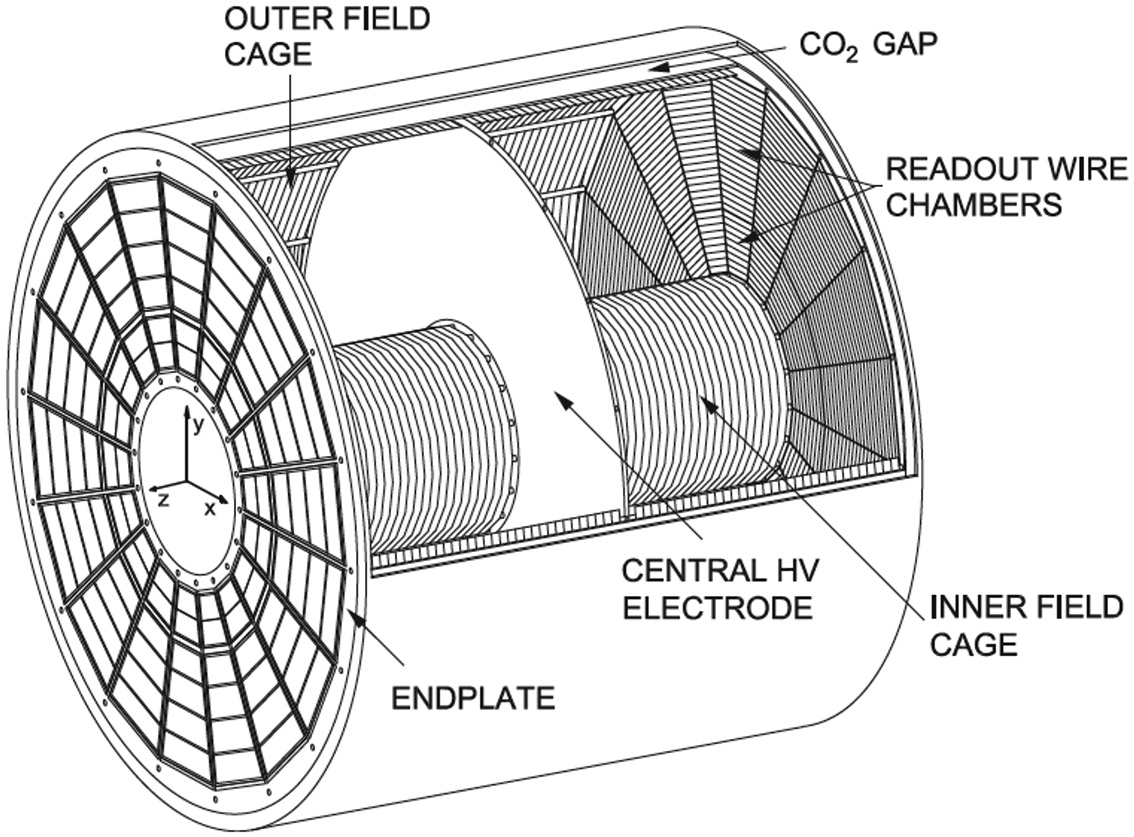
\includegraphics[width=0.8\textwidth]{figures/TPC.png}
    \caption[Schematic view of the Time Projection Chamber]{Scheme of a TPC. Sectors at the endplate detect electrons that are created by ionization of atoms. Taken from Ref.~\cite{sauli_2014}.}
    \label{df11}
\end{figure}
\FloatBarrier

\subsection{Time of Flight detector}
The TOF detector, as can be deduced from the name, measures the time of flight of particles which is then used for particle identification (PID). It is a fast detector with quick readout time which also is used as a trigger. TOF consists of 2 subsystems: the pseudo Vertex Position Detector (pVPD) and the Time of Flight patch (TOFp). pVPDs are located close the the beam line on each side of of the detector and work as a starting point in time for measurement. The TOFp is located around the TPC (exact locations can be seen in \autoref{df5}) and serves as a stopping mechanism for measuring time. pVPDs are plastic scintillators as well as the stop detector, TOFp, which consists of 120 trays. Each tray consists of 32 Multi-gap Resistive Plate Chambers (MRPCs) \cite{MRPC}. The principle of such detectors is that a traversing particle ionizes gas inside and the ejected electrons create electron avalanches (due to electric field) which create signal at the anode \cite{raphalthesis}. The time resolution is 60-100 ps. Part of the BES II upgrade done in 2019, was the expansion of $\eta$ range. The project stemmed from the collaboration of CBM and STAR and meant the installation of CBM modules on east side of the STAR detector. These modules measure range $-1.6<\eta <-1.1$ and their time resolution was measured to be around 83 ps \cite{BESII}. 

\FloatBarrier
\begin{figure}[ht]
    \centering
    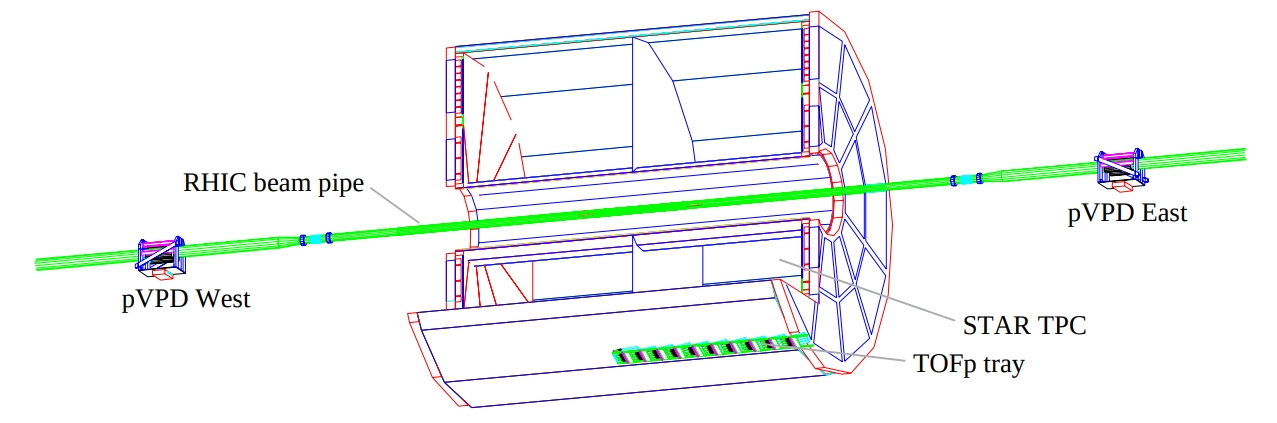
\includegraphics[width=0.9\textwidth]{figures/TOF.jpg}
    \caption[Schematic view of the Time Of Flight detector]{Scheme of Time of Flight detector around the TPC and positions of pseudo Vertex Position detectors which are located 5.6 m away from the center of STAR. Figure taken from Ref.~\cite{TOF}.}
    \label{df5}
\end{figure}
\FloatBarrier

\subsection{Roman Pot system}
\label{RPs}
Roman Pot system holds a crucial role in diffractive physics and detecting forward scattered protons. RPs are designed to measure the $(x,y,z)$ coordinates of protons which are used to reconstruct momenta. Momentum is mostly reconstructed in the transverse direction $(x,y)$. Thanks to the conservation of transverse momentum, such measurement helps to identify exclusive production. Altogether, there are 8 Roman Pots located around the STAR detector and are closely shown and described in \autoref{df6}. Each Roman Pot consists of 4 Silicon Strip Detectors (SSD) and a trigger scintillation counter. The active area of the detector is roughly $79 \times 49$ mm \cite{raphalmsc}. The average efficiency of a Roman Pot is approximately 99.98 $\%$ \cite{STAR}.

\FloatBarrier
\begin{figure}[ht]
    \centering
    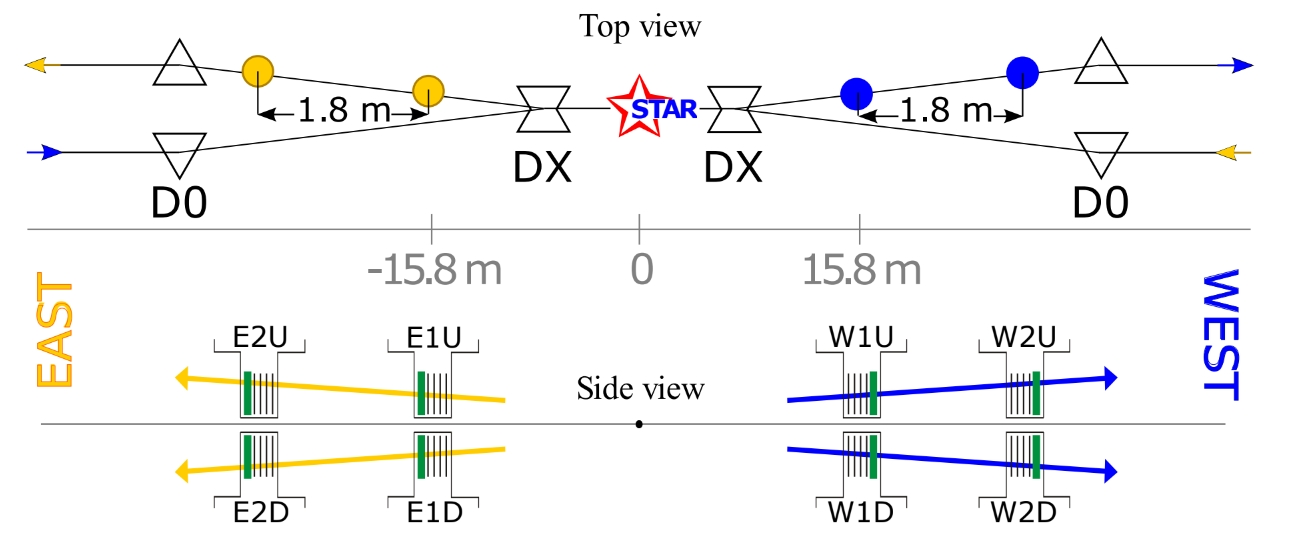
\includegraphics[width=0.85\textwidth]{figures/RP.jpg}
    \caption[Schematic view of the Roman Pot system]{Scheme of layout of the Roman pots. DX and D0 are magnets which curve the trajectories of the charged particles. Each Roman Pot is denoted with 3 different characters based on the position. E and W for east and west, 1 or 2 for position closer and further from the STAR detector, and U or D for up or down based on whether $y>0$ or $y<0$. The positions 1 and 2 are located 15.8 and 17.6 m away from the center of STAR. Taken from Ref.~\cite{raphalthesis}.}
    \label{df6}
\end{figure}
\FloatBarrier

\subsection{Beam Beam Counters}
Beam Beam counters are located on both sides of the cylindrical shape of TPC at around 3.75 m from the interaction point, as can be seen in \autoref{df4}. BBCs are plastic scintillators of hexagonal shape used mostly for providing minimum-bias trigger and for monitoring the collision rate \cite{raphalthesis}. They fall into 2 subcategories: large BBCs (or BBC-L) and small BBCs (or BBC-S). BBC-L cover the region $2.1<|\eta|<3.3$ and BBC-S range of $3.3<|\eta|<5.0$ \cite{STAR}. The time resolution of BBCs is approximately 900 ps \cite{Truhlar}.


\FloatBarrier
\begin{figure}[ht]
    \centering
    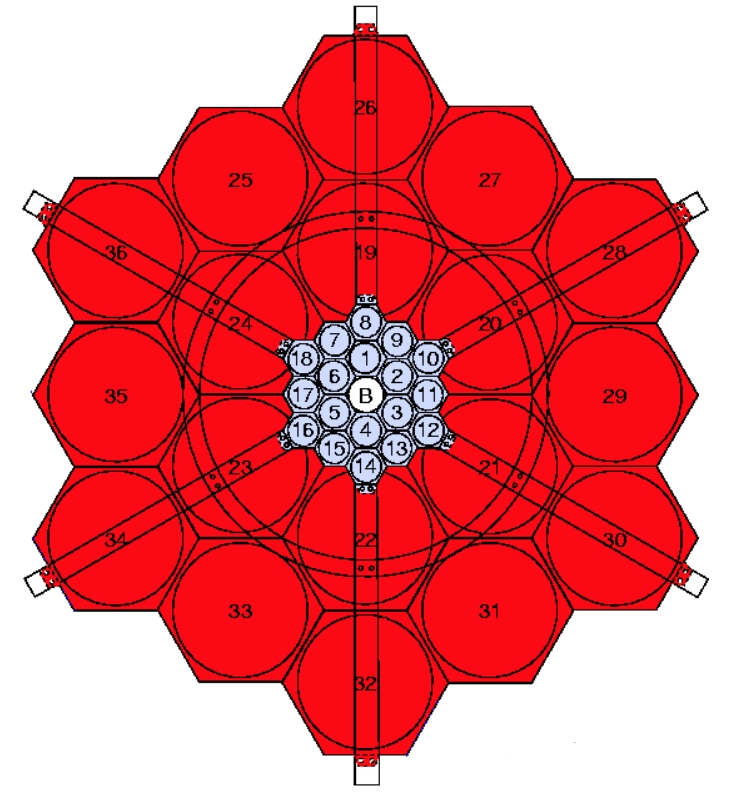
\includegraphics[width=0.6\textwidth]{figures/BBC.jpg}
    \caption[Schematic view of a Beam Beam Chamber]{Schematic view of BBC. Red hexagonal shapes represent the BBC-L, light blue are BBC-S and B in the middle stands for beam line. Taken from Ref.~\cite{STAR}.}
    \label{df7}
\end{figure}
\FloatBarrier

\subsection{Zero Degree Calorimeters}
ZDCs are hadron calorimeters that hold the purpose of detecting neutrons along the beam line. They are located on either side of the detector 18 m away from the interaction point behind the dipole magnets, which are denoted as DX in \autoref{df6}. Because ZDCs are measuring neutral particles, they are positioned at (x,y)=(0,0). The neutron multiplicity plays a significant role in determining the centrality\footnote{Centrality of a collision is determined by the geometry and the degree of overlap in collision and is used mostly in heavy ion collisions. A head-on collision means 0 $\%$ centrality and 2 nuclei missing each other means 100 $\%$ centrality.} of symmetric collisions as well as it provides a way of monitoring luminosity \cite{ZDC}. On each side of the STAR detector is located a ZDC which is constructed out of 3 modules. Each module consists of tungsten plates, fibers and photon multiplier tubes \cite{ZDC}.

\subsection{Other subsystems}
There are a few more parts which do not hold a significant role in analysis for the purpose of this thesis, yet they are worth mentioning. An interesting way of measuring energy of electromagnetic interaction are electromagnetic calorimeters. STAR has 2 of them: Barrel Electromagnetic Calorimeter\cite{BEMC} (BEMC) and Endcap Electromagnetic Calorimeter\cite{EEMC} (EEMC) which cover the full azimuthal angle with ranges of $|\eta|<1$ and $1<|\eta|<2$ respectively. The Muon Telescope Detector (MTD) was installed between the years 2012 and 2014 and is very efficient at identifying muons. This is crucial for identifying heavy quark states through the dilepton decay channel. The MTD covers about 45 $\%$ of the azimuthal angle and measures muons in the range $|\eta|<0.5$ \cite{MTD}. Another detector worth mentioning is Event Plane Detector (EPD) which was installed before run18, in 2018 \cite{BESII}. One on each side covers the range of pseudorapidity $2.1<|\eta|<5.1$. Their objective is to reconstruct event plane and provide information on the geometry of heavy nuclei collisions \cite{EPD}.

\FloatBarrier
\begin{figure}[ht]
    \centering
    \includegraphics[width=0.9\textwidth]{figures/fu.jpg}
    \caption[Schematic view of the STAR detector with highlighted forward upgrade BES II]{Scheme of the STAR detector with highlighted forward upgrade. Light and darker purple near the beam line represent the FTS and FCS. Taken from Ref.~\cite{BNL}.}
    \label{df10}
\end{figure}
\FloatBarrier

Part of the 2019 BES II focus was the forward upgrade. It included Forward Tracking System (FTS) and Forward Calorimeter System (FCS) which both cover the range $2.5<|\eta|<4$. The FTS consists of 4 small-strip Thin Gap Chambers (sTGC) which are capable of measuring transverse particles' momenta in range $0.2<p_T<2$ GeV/c with 20-30 $\%$ momentum resolution \cite{BESII}. The FCS includes a hadron as well as an electromagnetic calorimeter. Though there are a few more subordinate systems of the STAR detector, there is no capacity to discuss them in this thesis.

\section{EIC and the future}
\label{EIC}

The Electron-Ion Collider will be colliding heavy nuclei and protons with electrons which are significantly smaller and lighter. With sufficient energy, it means electrons will not be interacting with the nuclei as a whole, but with sole nucleons, quarks even. This might shine light onto the complex structures of nuclei, but also gluons, sea quarks and valence quarks which make up hadrons. It could uncover the saturation level of quarks that is called color glass condensate \cite{EIC}. Eventually, results from experiments at EIC will bring physicists closer to understanding the strong interaction. Electron-Ion Collider will improve the ability of RHIC to collide polarized protons (up to 70 $\%$), that will furthermore widen the knowledge of proton spin. This will be the first electron-ion collider in the world, therefore, significant results are expected. 
\FloatBarrier
\begin{figure}[ht]
    \centering
    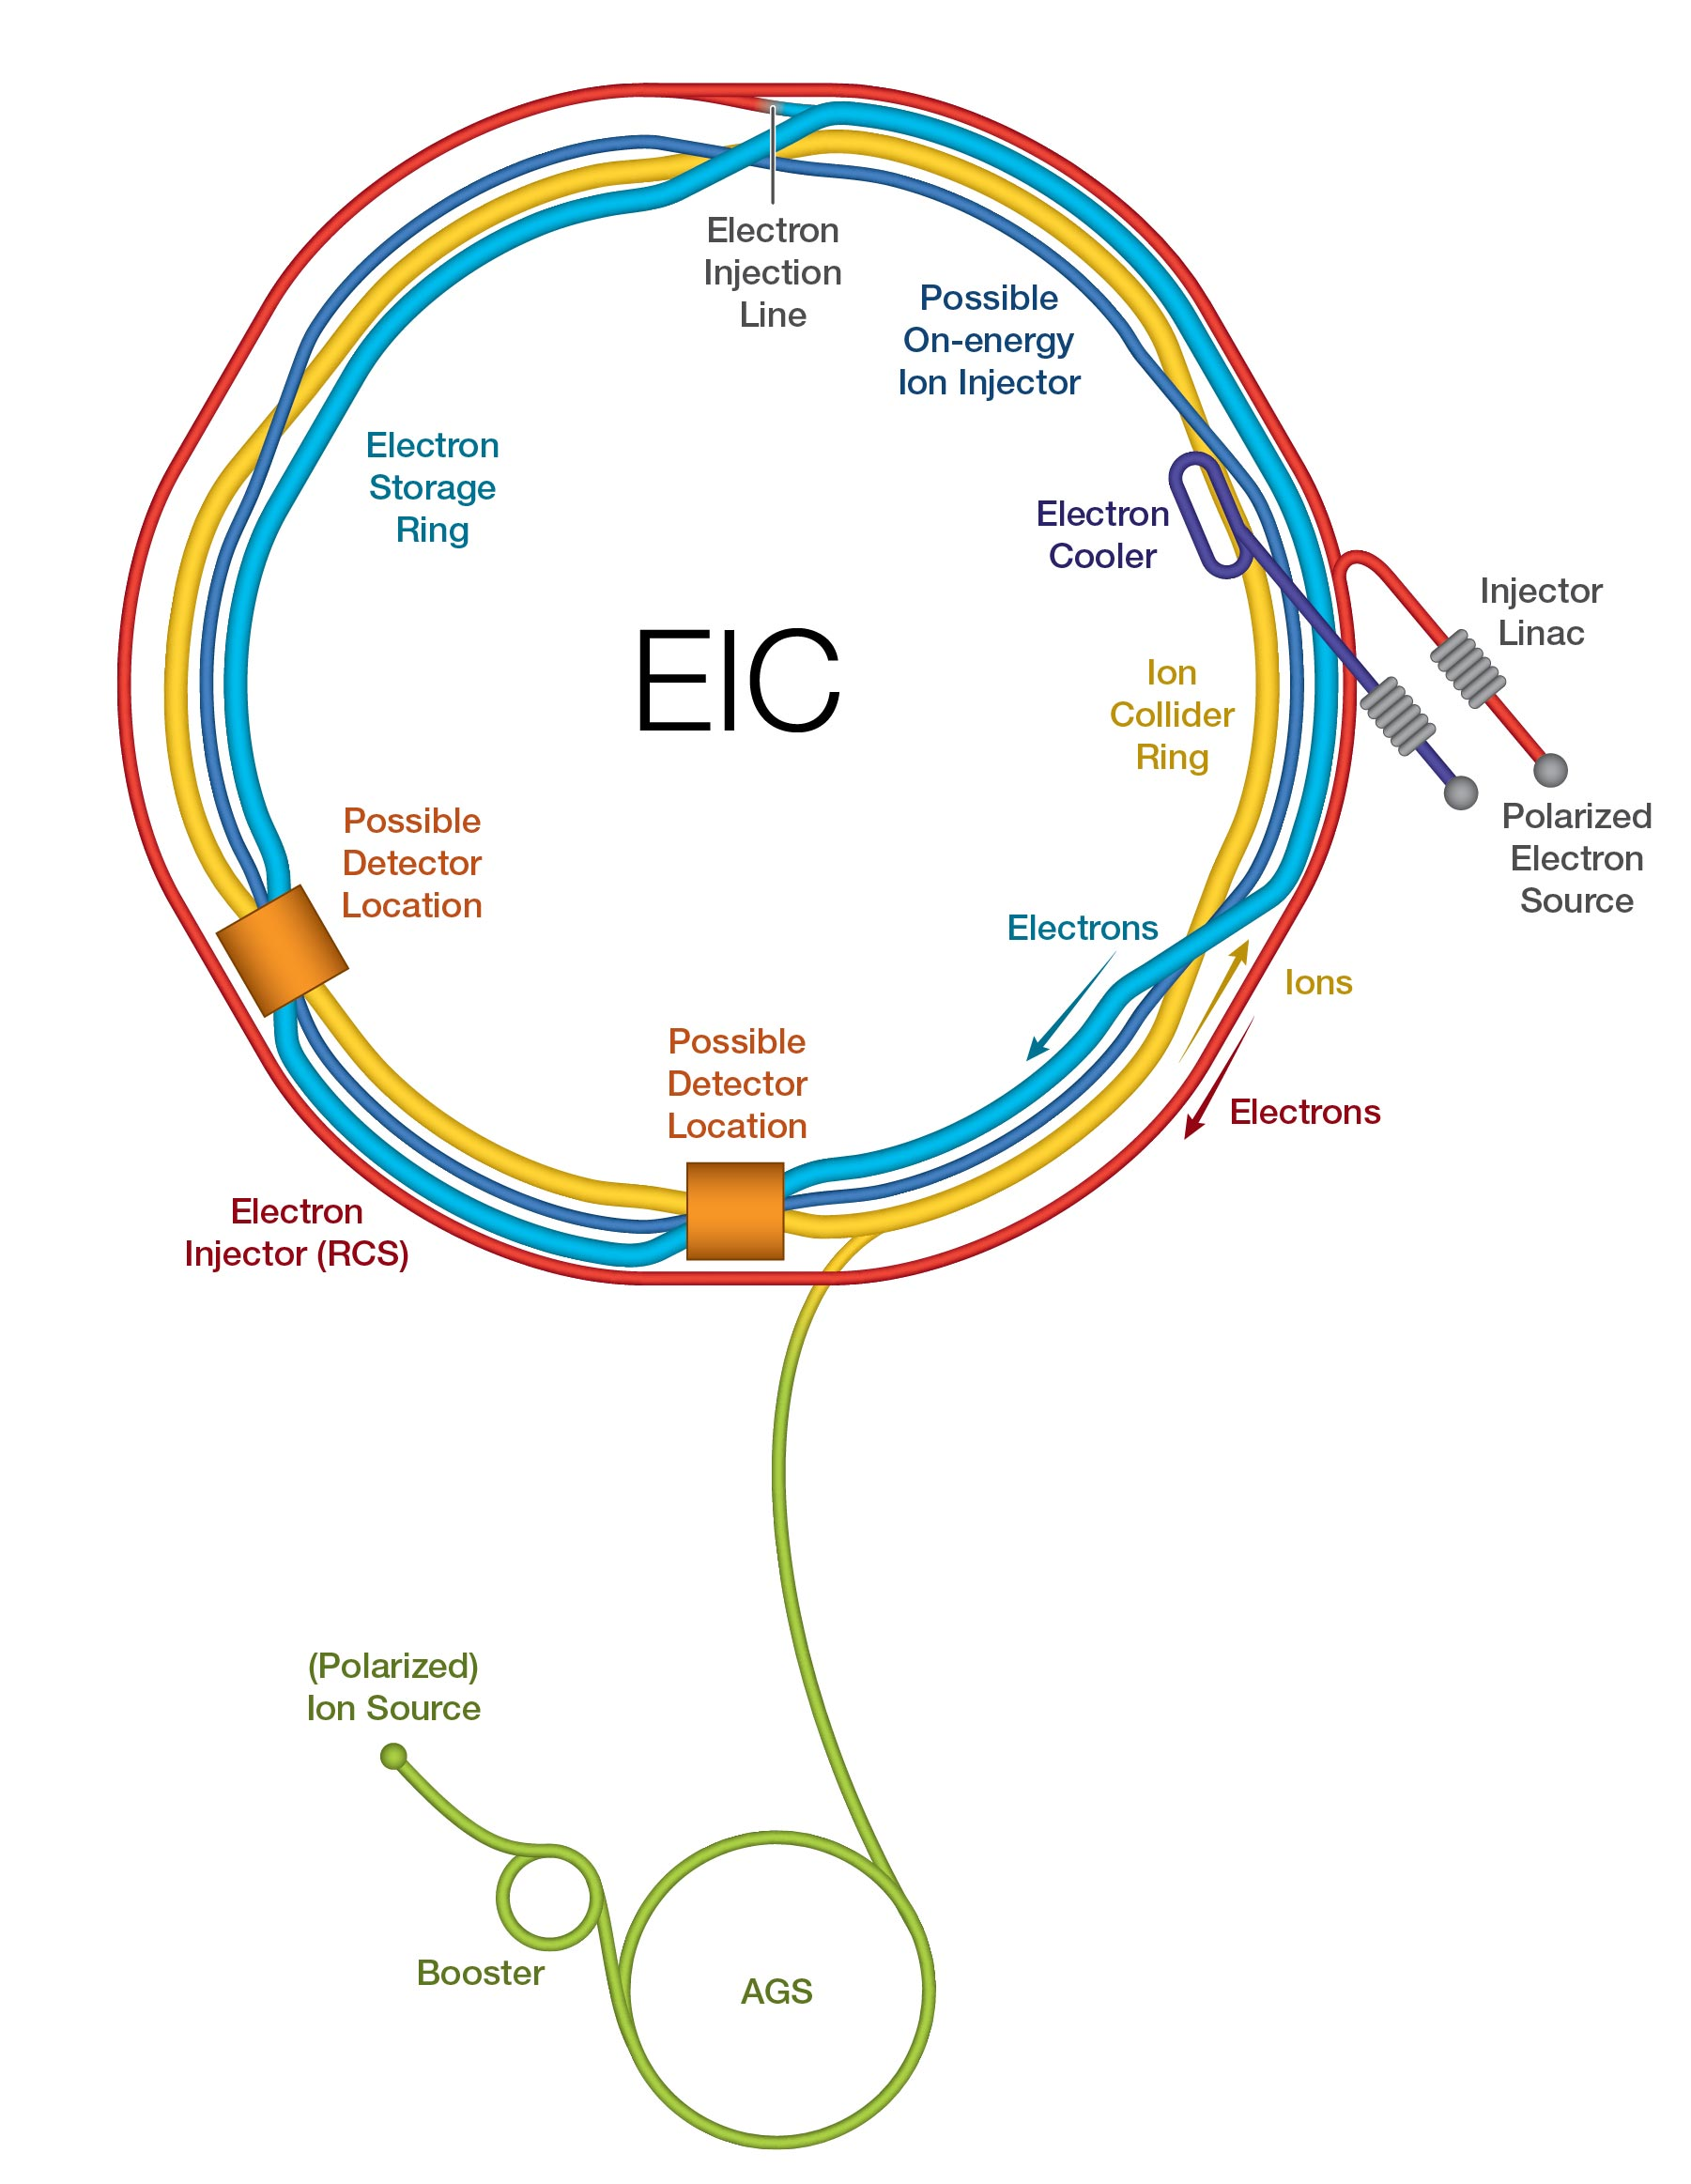
\includegraphics[width=0.7\textwidth]{figures/EIC.jpg}
    \caption[Schematic view of the Electron Ion Collider]{Scheme of the planned structure of Electron-Ion Collider at Brookhaven National Laboratory. Taken from Ref.~\cite{flickr}. }
    \label{df2}
\end{figure}
\FloatBarrier
EIC will be built in the tunnels of RHIC. It will make use of the RHIC's ion accelerators that are already implemented, but will require new electron sources and accelerators as well as a new electron storage ring \cite{EIC}. Even though construction begins after the end of operation of RHIC in 2025, many works have already begun. Simulations of collisions are already being made and detectors planned. The collider is expected to have at least 2 interaction points at which 2 detectors will be installed. The point of 2 or more detectors is their complementarity. It translates to the fact that breakthrough results done at one of the detectors can be researched on the other one, whether it means proving it right or discrediting it. On the other hand, results from 2 different independent detectors hold higher significance. The proposals and ideas for second detector at the EIC were to begin in 2023.
\newline
Although the concept of an ideal detector for electron-ion collisions is something that has not been studied before, a big source of knowledge comes from collider HERA, which facilitated electron-proton collisions. The asymmetry of the collisions will mean very different particle distributions from those, that can be seen at the STAR experiment. The goal is to combine all the requirements with the best technology and material all the while staying within a certain budget. 
\FloatBarrier
\begin{figure}[ht]
    \centering
    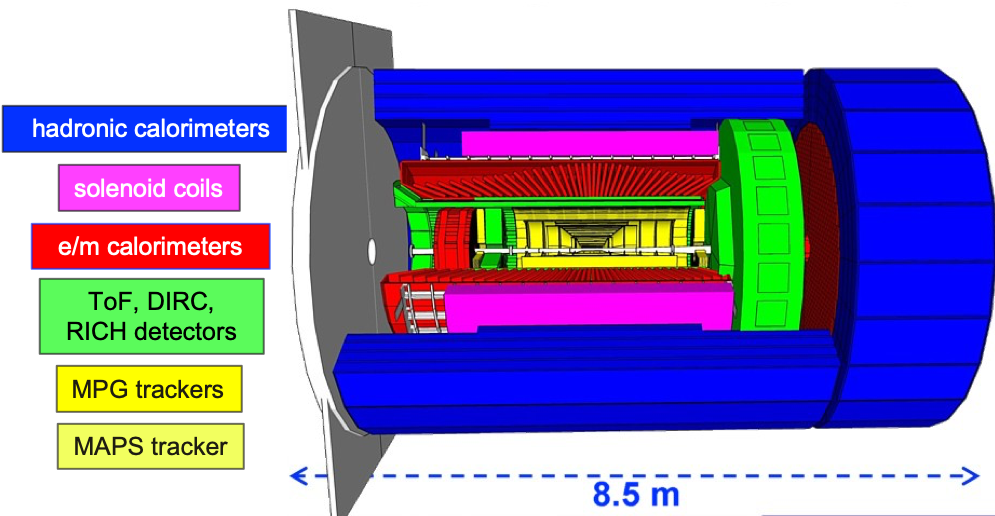
\includegraphics[width=0.9\textwidth]{figures/epic.png}
    \caption[Schematic view of the ePIC detector]{Crosscut view of the ePIC detector planned to be built at the EIC. Taken from Ref.~\cite{EIC}.}
    \label{df3}
\end{figure}
\FloatBarrier
The design of such detector focuses on tracking and vertexing, particle identification, calorimetry systems and endcap detectors \cite{EICdetectorrequirements}. Tracking and vertexing will be done using a double-sided time projection chamber, gas electron multipliers (GEM), $\mu$MEGA, that can be used for tracking neutrons, or $\mu$RWELL (more in Ref.~\cite{muWELL}) which all are high precision gas detectors. At the moment, the best material for vertex tracking is silicon, which is why all the tracking detectors will be made from this material \cite{Higinbotham}. Particle identification relies highly on ionization trails from TPC, but there will be additional detectors which are based on the principle of Cherenkov radiation such as a dual and modular Ring Imaging Cherenkov Detector (dRICH and RICH) and internally reflected Cherenkov light detectors \cite{EICdetectorrequirements}. The measurement of energy of particles will be provided through electromagnetic (ECAL) and hadron (HCAL) calorimeters. The exact types with specific properties are still under study. In addition to the detector of the central region, auxiliary detectors for forward and backward regions will be installed. Roman pots for far-forward tagging, ZDCs for detecting neutrons and low-energy photons will be installed as well as some other detectors that have not been chosen yet. Polarimeters, detectors that measure polarization, will be installed in several sections of the EIC \cite{EICdetectorrequirements}. All of the detectors which will be part of the Electron-Ion Collider are currently being tested at Thomas Jefferson National Accelerator Facility. Jefferson lab is another laboratory under the administration of U.S. Department of Energy and is located in Virginia, U.S. EIC is expected to begin running in the early 2030s.
